\documentclass[a4paper, 12pt]{article}
\usepackage[utf8]{inputenc}
\usepackage[russian,english]{babel}
\usepackage[T2A]{fontenc}
\usepackage[left=10mm, top=20mm, right=18mm, bottom=15mm, footskip=10mm]{geometry}
\usepackage{indentfirst}
\usepackage[yyyymmdd,hhmmss]{datetime}

\usepackage{graphicx}

\usepackage{titlesec}
\usepackage{parskip}

\usepackage{graphicx}
\graphicspath{{images/}}
\DeclareGraphicsExtensions{.pdf,.png,.jpg,.bmp}

\usepackage{wrapfig}
\usepackage{blindtext}
\usepackage{cmap}

\usepackage[x11names]{xcolor}

\usepackage{amsmath} % math packages
\usepackage{amsfonts}
\usepackage{amsmath}
\usepackage{amssymb}
\usepackage{amsthm}
\usepackage{mathtools}

\usepackage{uniquecounter}
\usepackage{placeins}
\usepackage[italicdiff]{physics}

\usepackage{multirow}

\usepackage{hyperref} % links in document
\hypersetup{
    colorlinks=true,
    linkcolor=red,
    filecolor=magenta,      
    urlcolor=blue,
    pdftitle={Links},
    pdfpagemode=FullScreen,
}

\usepackage{import} %inkspace images
\usepackage{xifthen}
\usepackage{pdfpages}
\usepackage{transparent}

\usepackage{caption}
\captionsetup[figure]{name=Рисунок}
\captionsetup[table]{name=Таблица}

\usepackage{fancyhdr}

\title{Определение $C_p$/$C_v$ по скорости звука в газе (2.1.3)}
\author{Хмельницкий Антон Б01-306}
\date{\today}

\begin{document}

    \maketitle
    \section{Теоретические сведения}
	
	Скорость распространения звуковой волны в газах зависит от показателя адиабаты $\gamma $. На измерении скорости звука основан один из наиболее точных методов определения показателя адиабаты.
	
	Скорость звука в газах определяется формулой:
	
	\begin{equation}
		c=\sqrt{\gamma\frac{RT}{\mu}}.
		\label{velocity}
	\end{equation}
	где $ R $ -- газовая постоянная, $ T $ -- температура газа, а $ \mu $ -- его молярная масса. Преобразуя эту формулу, найдем
	\begin{equation}\label{gamma}
		\gamma = \frac{\mu}{RT}c^2.
	\end{equation}

    Условия стоячей волны
    \[ L=n\lambda/2, \] где $ \lambda $ -- длина волны звука в трубе, а $ n $ -- любое целое число.
	
	Скорость звука c связана с его частотой $ f $ и длиной волны $ \lambda $ соотношением
	
	\begin{equation}\label{lambda_f}
		c=\lambda f.
	\end{equation}
	
	Подбор условий, при которых возникает резонанс, можно производить двояко:
	\begin{enumerate}
		\item При неизменной частоте $ f $ звукового генератора (а следовательно, и неизменной длине звуковой волны $ \lambda $) можно изменять длину трубы $ L $. Для этого применяется раздвижная труба. Длина раздвижной трубы постепенно увеличивается, и наблюдается ряд последовательных резонансов. Возникновение резонанса легко наблюдать на осциллографе по резкому увеличению амплитуды колебаний. Для последовательных резонансов имеем \begin{equation}\label{first}
			L_n=n\frac{\lambda}{2}, \quad L_{n+1}=(n+1)\frac{\lambda}{2}, \quad \dots, \quad L_{n+k} = n\frac{\lambda}{2}+k\frac{\lambda}{2},
		\end{equation} т. е. $ \lambda/2 $ равно угловому коэффициенту графика, изображающего зависимость длины трубы $ L $ от номера резонанса $ k $. Скорость звука находится по формуле \eqref{lambda_f}.
		\item При постоянной длине трубы можно изменять частоту звуковых колебаний. В этом случае следует плавно изменять частоту $ f $ звукового генератора, а следовательно, и длину звуковой волны $ \lambda $. Для последовательных резонансов получим 
		\begin{equation}\label{4}
			L=\frac{\lambda_1}{2}n=\frac{\lambda_2}{2}(n+1)=\dots=\frac{\lambda_{k+1}}{2}(n+k).
		\end{equation}
		
		Из \eqref{lambda_f} и \eqref{4} имеем:
		\[ f_1=\frac{c}{\lambda_1}=\frac{c}{2L}n, \quad f_2=\frac{c}{\lambda_2}=\frac{c}{2L}(n+1)=f_1+\frac{c}{2L},\quad \dots, \]
		\begin{equation}\label{5}
			f_{k+1}=\frac{c}{\lambda_{k+1}}=\frac{c}{2L}(n+k)=f_1+\frac{c}{2L}k.
		\end{equation}
	\end{enumerate}    

\section{Расчет всех данных}

\begin{table}[!h]
\begin{center}
\caption{Данные установки с термостатом для воздуха}
\begin{tabular}{|c|c|c|c|c|c|c|c|c|c|c|c|c|}
\hline
Воздух 1     & $\nu_1$ & T    & 25,3 & $\nu_2$ & T    & 40 & $\nu_3$ & T    & 45 & $\nu_4$ & T    & 52 \\ \hline
$L$ = 800 мм & 1       & 202  &      & 1      & 205  &    & 1      & 208  &    & 1      & 209  &    \\ \hline
             & 2       & 450  &      & 2      & 461  &    & 2      & 464  &    & 2      & 469  &    \\ \hline
             & 3       & 660  &      & 3      & 677  &    & 3      & 682  &    & 3      & 689  &    \\ \hline
             & 4       & 874  &      & 4      & 896  &    & 4      & 903  &    & 4      & 913  &    \\ \hline
             & 5       & 1088 &      & 5      & 1118 &    & 5      & 1127 &    & 5      & 1139 &    \\ \hline
\end{tabular}
\end{center}
\end{table}

\begin{table}[!h]
\begin{center}
\begin{tabular}{|l|l|l|l|l|l|}
\hline \multicolumn{2}{|l|}{$\mathrm{\nu}=4412$ Гц} & \multicolumn{2}{|l|}{$\mathrm{\nu}=3707$ Гц} & \multicolumn{2}{|l|}{$\mathrm{\nu}=5092$ Гц}\\ \hline 
$\mathrm{k}$ & $\mathrm{dL}$, мм & $\mathrm{k}$ & $\mathrm{dL}$, мм & $\mathrm{k}$ & $\mathrm{dL}$, мм  \\ \hline 
0 & 20 & 0 & 36 & 0 & 8 \\ \hline 
1 & 55 & 1 & 87 &  1 & 41  \\ \hline 
2 & 96 & 2 & 129 &  2 & 76  \\ \hline 
3 & 131 & 3 & 180 & 3 & 109  \\ \hline 
4 & 172 & 4 & 220 & 4 & 143  \\ \hline
\end{tabular}
\caption{Данные установки с выдвижной частью для воздуха}
\end{center}
\end{table}

\begin{table}[!h]
\begin{center}
\begin{tabular}{|l|l|l|l|l|l|l|l|l|l|}
\hline \multicolumn{2}{|l|}{$\mathrm{\nu}=4398$ Гц} & \multicolumn{2}{|l|}{$\mathrm{\nu}=3506$ Гц} & \multicolumn{2}{|l|}{$\mathrm{\nu}=3039$ Гц} \\
\hline $\mathrm{k}$ & $\mathrm{dL}$, мм & $\mathrm{k}$ & $\mathrm{dL}$, мм & $\mathrm{k}$ & $\mathrm{dL}$, мм  \\
\hline 0 & 52 & 0 & 47 & 0 & 50 \\
\hline 1 & 81 & 1 & 86 & 1 & 94 \\
\hline 2 & 112 & 2 & 124 & 2 & 138 \\
\hline 3 & 143 & 3 & 163 & 3 & 182 \\
\hline 4 & 173 & 4 & 199 & 4 & 226  \\
\hline
\end{tabular}
\caption{Данные установки с выдвижной частью для углекислого газа}
\end{center}
\end{table}

\section{Обработка резальтатов}

Расчет погрешность при аппроксимации по МНК:

\[k=\frac{\langle xy\rangle-\langle x\rangle \langle y\rangle}{\langle x^2\rangle - \langle x\rangle^2}\]
\[b = \langle y \rangle - k \langle x \rangle\]
\[\sigma_{k} = \frac{1}{\sqrt{N}}\sqrt{\frac{\langle y^2 \rangle - \langle y \rangle ^2}{\langle x^2 \rangle - \langle x \rangle ^2} - k^2}\]
\[\sigma_{b} = \sigma_{k}\sqrt{\langle x^2 \rangle}\]

Для $\Delta f = f_{k+1} - f_{1}= \frac{c}{2L}k$:
\[\gamma = \frac{\mu}{RT}c^2 = \frac{4L^2k^2\mu}{RT}\]
\newline
\[T_1 = 298,3 K\]
\[k_1 = 219.6, \gamma_1 = 1,44\]
\[\sigma_{k_1} = 3.069 (\varepsilon = 1,4\%)\]
\[b_1 = 13.6\]
\[\sigma_{b_1} = 7.5\]

\[T_2 = 313 K\]
\[k_2 = 226.6, \gamma_2 = 1,47(\varepsilon = 1,41\%)\]
\[\sigma_{k_2} = 3.2\]
\[b_2 = 14.2\]
\[\sigma_{b_2} = 7.85\]

\[T_3 = 318 K\]
\[k_3 = 227.7, \gamma_3 = 1,46(\varepsilon = 1,3\%)\]
\[\sigma_{k_3} = 3.02\]
\[b_3 = 13.4\]
\[\sigma_{b_3} = 7.4\]

\[T_4 = 325 K\]
\[k_4 = 230.4, \gamma_4 = 1,45(\varepsilon = 1,37\%)\]
\[\sigma_{k_4} = 3.16\]
\[b_4 = 13.9\]
\[\sigma_{b_4} = 7.74\]

Для $\Delta L = L_{k+1} - L_{1}= \frac{\lambda}{2}k$ у воздуха:
\[\gamma = \frac{\mu}{RT}c^2 = \frac{4f^2k^2\mu}{RT}, T = 298,3 K\]
\[f_1 = 5092\]
\[k_1 = 0,035, \gamma_1 = 1,5(\varepsilon = 2,3\%)\]
\[\sigma_{k_1} = 0,0008\]
\[b_1 = -0,05\]
\[\sigma_{b_1} = 4\]

\[f_2 = 4412\]
\[k_2 = 0,045, \gamma_2 = 1,75(\varepsilon = 1,5\%)\]
\[\sigma_{k_2} = 0,0007\]
\[b_2 = -0,003\]
\[\sigma_{b_2} = -0,0004\]

\[f_3 = 5092\]
\[k_3 = 0,033, \gamma_3 = 1,32(\varepsilon = 2,7\%)\]
\[\sigma_{k_3} = 0.0009\]
\[b_3 = -0.01\]
\[\sigma_{b_3} = 0.005\]

Для $\Delta L = L_{k+1} - L_{1}= \frac{\lambda}{2}k$ у $CO_2$:
\[\gamma = \frac{\mu}{RT}c^2 = \frac{4f^2k^2\mu}{RT}, T = 298,3 K\]
\[f_1 = 5092\]
\[k_1 = 0,033, \gamma_1 = 1,33\]
\[\sigma_{k_1} = 0,001(\varepsilon = 3\%)\]
\[b_1 = 0,01\]
\[\sigma_{b_1} = 0,004\]

\[f_1 = 4398\]
\[k_1 = 0,039, \gamma_2 = 1,39(\varepsilon = 1,5\%)\]
\[\sigma_{k_1} = 0,0006\]
\[b_1 = 0,003\]
\[\sigma_{b_1} = 0,0002\]

\[f_3 = 3506\]
\[k_3 = 0,044, \gamma_3 = 1,2(\varepsilon = 1\%)\]
\[\sigma_{k_3} = 0.0004\]
\[b_3 = 0.0002\]
\[\sigma_{b_3} = 0.00005\]

\section{Вывод}

Сравнивая реузльтаты получаем среднее значение показателя адиабаты на 1 установке $\gamma = 1,44 \pm 0,0197 (\varepsilon_{sr} = 1,37\%)$, на второй $\gamma = 1.33 \pm 0,027 (\varepsilon_{sr} = 2\%)$.
Сравнивая с табличным, получаем погрешность 1,4\%, на второй 2\%, что подтверждает точность метода измерения с помощью скорости звука в воздухе изменение от температуры и типа воздуха.

\newpage

\begin{figure}[!p]
    \centering
    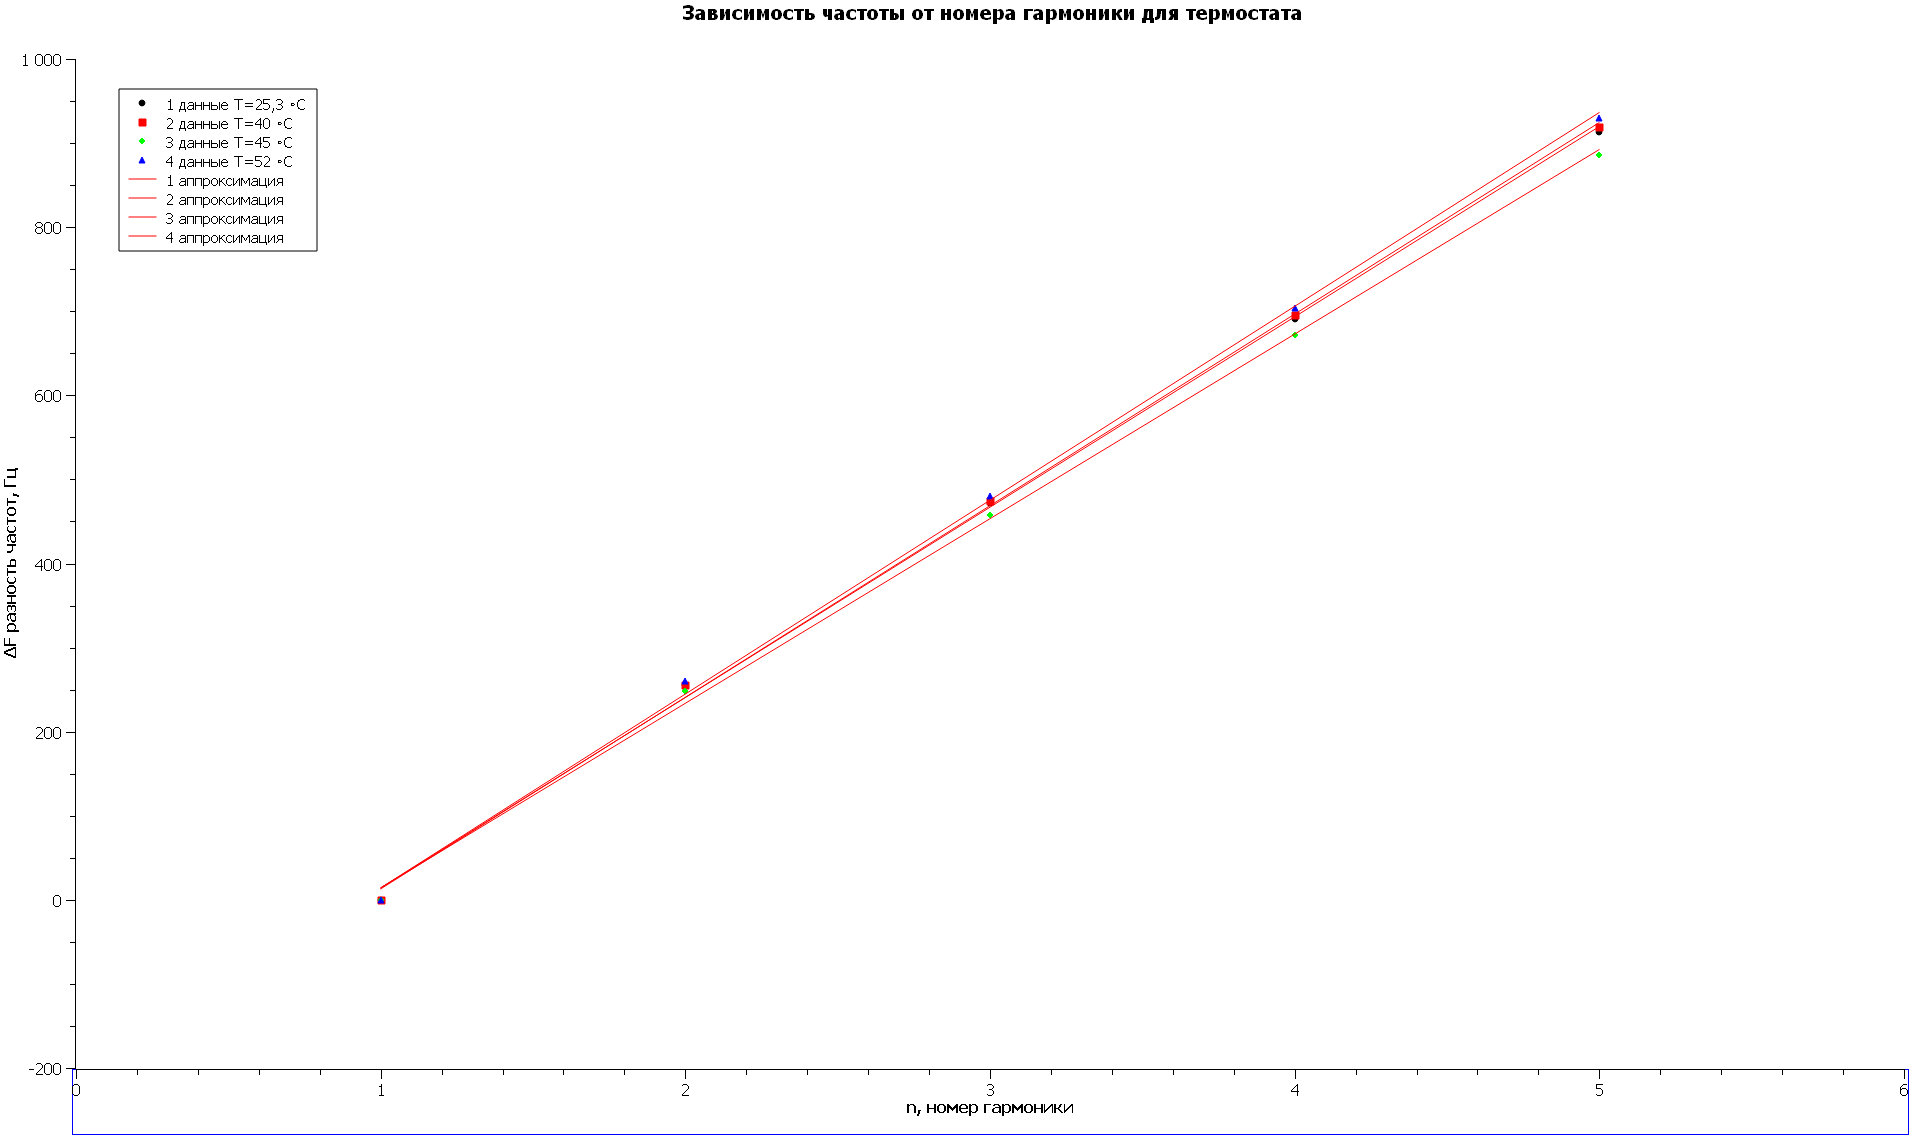
\includegraphics[width=0.9\textwidth]{graphic1.png}
    \caption{Длина от номера гармоники для воздуха}
\end{figure}

\begin{figure}[!p]
    \centering
    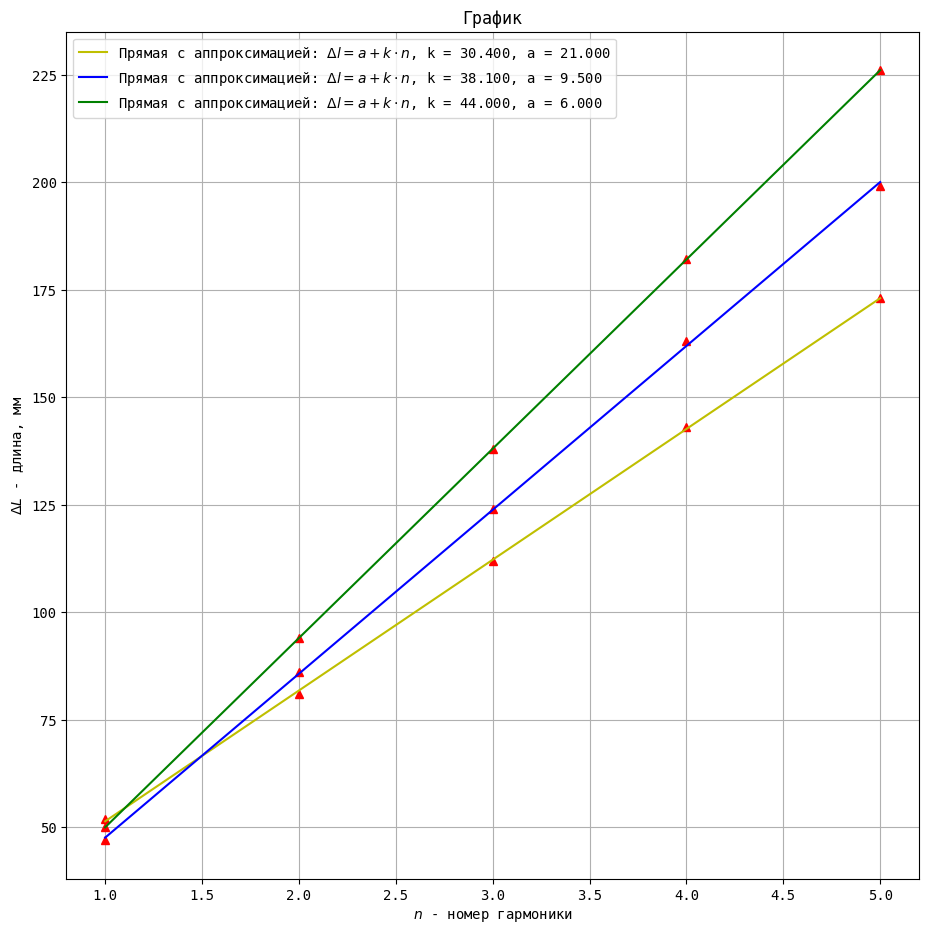
\includegraphics[width=0.9\textwidth]{graphic2.png}
    \caption{Длина от номера гармоники для $CO_2$}
\end{figure}

\begin{figure}[!p]
    \centering
    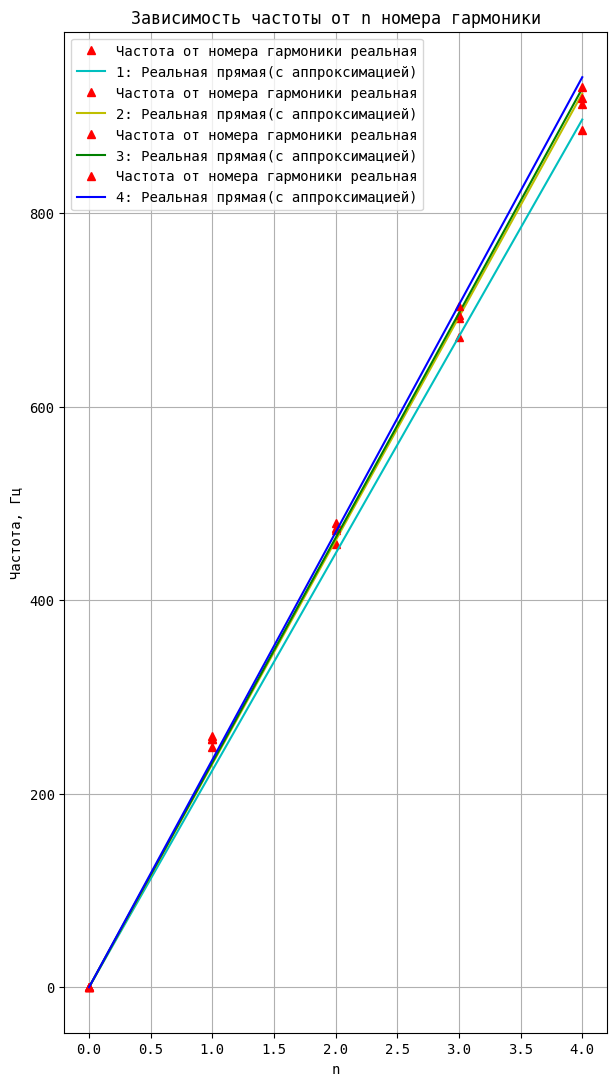
\includegraphics[width=0.8\textwidth]{graphic.png}
    \caption{Частота от номера гармоники для воздуха при разных температурах}
\end{figure}

\end{document}